\documentclass[12pt,a4paper]{memoir}
% \documentclass[titlepage,12pt,a4paper]{book}

\usepackage{acro}
\acsetup{first-style=short}
\usepackage[portuguese]{babel}
\usepackage[utf8]{inputenc}
\usepackage[T1]{fontenc}
\usepackage{makeidx}
\usepackage{xspace}
\usepackage{graphicx, color, times}
\usepackage{fancyhdr}
\usepackage{pxfonts}
\usepackage{times}
\usepackage{amssymb}
\usepackage{amsfonts}
\usepackage{amsmath}
\usepackage{latexsym}
%\usepackage[printonlyused]{acronym}
\usepackage{float}
\usepackage{listings}
\usepackage{tocbibind}
\usepackage{natbib}
\usepackage[hidelinks]{hyperref}
\usepackage[T1]{fontenc}
\usepackage{titlesec, blindtext, color}
\usepackage{url}
\usepackage[acronym]{glossaries}
\usepackage{listings}


% \renewcommand{\ttdefault}{phv}

\pagestyle{fancy}
\renewcommand{\chaptermark}[1]{\markboth{#1}{}}
\renewcommand{\sectionmark}[1]{\markright{\thesection\ #1}}
\fancyhf{} \fancyhead[LE,RO]{\bfseries\thepage}
\fancyhead[LO]{\bfseries\rightmark}
\fancyhead[RE]{\bfseries\leftmark}
\renewcommand{\headrulewidth}{0.5pt}
\renewcommand{\footrulewidth}{0pt}
\setlength{\headheight}{10pt}
\setlength{\marginparsep}{0cm}
\setlength{\marginparwidth}{0cm}
\setlength{\marginparpush}{0cm}
\addtolength{\hoffset}{-1cm}
\addtolength{\oddsidemargin}{\evensidemargin}
\addtolength{\oddsidemargin}{0cm}
\addtolength{\evensidemargin}{0.5cm}

\chapterstyle{box}

\usepackage{fix-cm}
\usepackage{fourier}
\usepackage[scaled=.92]{helvet}
\definecolor{ChapGrey}{rgb}{0.6,0.6,0.6}
\newcommand{\LargeFont}{
  \usefont{\encodingdefault}{\rmdefault}{b}{n}
  \fontsize{60}{80}\selectfont\color{ChapGrey}
  }
\makeatletter
\newcommand{\hsp}{\hspace{20pt}}

\makeatother
\chapterstyle{GreyNum}

\setcounter{tocdepth}{3}
\setsecnumdepth{subsubsection}

\renewcommand{\ttdefault}{lmtt}

% cores
\definecolor{gray75}{gray}{0.75}
\definecolor{dark}{gray}{0.25} 
\definecolor{lgray}{gray}{0.9}
\definecolor{dkblue}{rgb}{0,0.13,0.4}
\definecolor{dkgreen}{rgb}{0,0.6,0}
\definecolor{gray}{rgb}{0.5,0.5,0.5}
\definecolor{mauve}{rgb}{0.58,0,0.82}

\lstset{ %
  language=SQL,                    basicstyle=\footnotesize,
  numbers=none,                  numberstyle=\tiny\color{gray}, 
  stepnumber=1,                  numbersep=5pt,
  backgroundcolor=\color{white}, showspaces=false,
  showstringspaces=false,        showtabs=false,
  frame=single,                  rulecolor=\color{black},
  tabsize=2,                     captionpos=b,
  breaklines=true,               breakatwhitespace=false,
  title=\lstname,                keywordstyle=\color{blue},
  commentstyle=\color{dkgreen},  stringstyle=\color{mauve},
  escapeinside={\%*}{*)},        morekeywords={*},
  belowskip=0cm
}

\renewcommand{\lstlistingname}{Excerto de Código}
\renewcommand{\lstlistlistingname}{Lista de Excertos de Código}

\renewcommand{\today}{\day \ifcase \month \or Janeiro\or Fevereiro\or Março\or %
Abril\or Maio\or Junho\or Julho\or Agosto\or Setembro\or Outubro\or Novembro\or %
Dezembro\fi de \number \year} 

\titleformat{\chapter}[hang]{\Huge\bfseries}{\thechapter\hsp\textcolor{gray75}{/}\hsp}{0pt}{\Huge\bfseries\slshape}
\titleformat{\section}[hang]{\Large\bfseries}{\thesection\hsp\textcolor{gray75}{|}\hsp}{0pt}{\Large\bfseries}

\newacronym{LaTeX}{LaTeX}{LAMBDA}
\newacronym{PDF}{PDF}{Portable Document Format}

\begin{document}

\include{capa}

\thispagestyle{empty}
\setcounter{page}{-1}

\begin{center}
\begin{Huge}
\textbf{Universidade da Beira Interior}
\end{Huge}
\end{center}

\begin{center}
\begin{Huge}
Departamento de Informática
\end{Huge}
\end{center}

\vspace{0,07cm}
\begin{figure}[!htb]
\centering

\includegraphics[width=191pt]{ubi-fe-di.png}
\end{figure}


\vspace{0.5cm}
\begin{center}
\begin{Large}
\textbf{\emph{Nome}}
\end{Large}
\end{center}


\vspace{0.5cm}
\begin{center}
\begin{normalsize}
\begin{large}
Elaborado por:
\end{large}
\end{normalsize}
\end{center}

\begin{center}
\begin{large}
\textbf{Tiago Ramos 47883 \\ Ricardo Matias 46586 \\ Daniel Oliveira 48118 \\ Francisco Gordino 48531} \\
\end{large}
\end{center}

\vspace{0,5cm}
\begin{center}
\begin{normalsize}
\begin{large}
Orientador:
\end{large}
\end{normalsize}
\end{center}

\begin{center}
\begin{large}
\textbf{Professor Doutor Abel Gomes}
\end{large}
\end{center}



\vspace{0.5cm}
\begin{center}
\begin{normalsize}
9 de Janeiro
\end{normalsize}
\end{center}

\clearpage{\thispagestyle{empty}\cleardoublepage}

\frontmatter

\acresetall

\include{agradecimentos}

\chapter*{Agradecimentos}
\label{chap:agradec}
\paragraph{} 
Agredecemos primeiramente ao nosso professor, D. Abel Gomes, pela oportunidade de podermos ampliar o nosso conhecimento na área de Computação Gráfica e também por podermos interagir com a linguagem C++ e com as bibliotecas do OpenGL, durante a realização deste trabalho assim como ao longo do semestre de modo a termos uma experiência mais técnica e próxima da realidade. \\

A sua abordagem didática, aliada à sua experiência na área, proporcionou um ambiente propício para o crescimento acadêmico e profissional de cada membro do grupo. Para além disso gostariamos de deixar uma palavra de agradecimento aos nossos colegas de curso, pelas discussões saudáveis e ajuda fornecida em quaisquer dúvidas que tenham surgido e podessem ser debatidas de modo a interagirmos para um bem comum.\\

A todo o incentivo e apoio prestado, é guardado connosco em sentido de
gratidão e cooperação.
\clearpage{\thispagestyle{empty}\cleardoublepage}

\include{resumo}



\clearpage{\thispagestyle{empty}\cleardoublepage}

\include{acronimos}

\chapter*{Acrónimos}
\label{chap:acro}
UBI - Universidade da Beira Interior\\
CG - Computação Gráfica\\
UC - Unidade Curricular\\
\printglossaries

\newpage
\tableofcontents



\mainmatter

\include{introducao}

\chapter{Motivação}
\label{chap:intro}
\label{sec:mot}
\paragraph{}
Motivados por um semestre sob a orientação do Professor Doutor Abel Gomes, durante o qual fomos guiados no desenvolvimento de trabalhos e tarefas, adquirimos conhecimentos fundamentais sobre desenvolvimento gráfico. Sentindo a necessidade de aplicar todo o aprendizado adquirido, não poderíamos encontrar desafio mais adequado do que o presente projeto.

\section{Objetivos}
\label{sec:obj}
\paragraph{}
Este projeto visa desenvolver uma representação gráfica do sistema solar por meio do OpenGL, em conjunto com diversas ferramentas e bibliotecas correlatas. A programação em C++ integra conceitos de renderização, manipulação de objetos e texturas, controles de câmera, e a utilização de shaders para criar uma experiência visual envolvente. Em projetos desse tipo, a aspiração comum é alcançar uma representação que se equipare a uma fotografia ou visão realista. Embora essa meta ainda não seja completamente atingida, a evolução nessa área está em constante avanço.

O tema selecionado para este projeto é a representação do sistema solar, aproveitando as ferramentas mencionadas para se aproximar ao máximo do objetivo proposto. A implementação apresenta uma aplicação interativa do sistema solar em escala, incorporando características realistas como rotação e órbita dos planetas. Este relatório explora diversos conceitos fundamentais, desde a configuração inicial do projeto até a renderização individual de cada planeta. Adicionalmente, são discutidas as estratégias adotadas para o controle de entrada do usuário, assim como a implementação de conceitos-chave, como transformações de matrizes e carregamento de texturas.

\newpage



\include{capitulo-2}

\chapter{Tecnologias Utilizadas}
\label{chap:Desenvolvimento}

\section{Visual Studio Code}
\label{chap2:sec:vscode}

O Visual Studio Code é um ambiente de desenvolvimento leve e poderoso da Microsoft, conhecido por sua interface intuitiva e flexibilidade. Sua aparência limpa e moderna oferece uma experiência visual agradável. Destaca-se pela extensibilidade, permitindo aos usuários personalizarem o ambiente com diversas extensões. Oferece recursos avançados de edição de código, como destaque de sintaxe e sugestões inteligentes. Suporta integração com várias linguagens de programação, controle de versão e ferramentas de automação, tornando-o uma escolha popular entre os desenvolvedores.



\section{C++}
\label{chap2:sec:c++}
\paragraph{}
C++ é uma linguagem de programação poderosa e amplamente utilizada, conhecida por sua eficiência e versatilidade. Projetada como uma extensão da linguagem C, o C++ oferece recursos adicionais, incluindo programação orientada a objetos, manipulação de memória e suporte para programação genérica.

Sua sintaxe é reconhecida por ser acessível aos programadores familiarizados com C, ao mesmo tempo em que introduz construções mais avançadas. C++ é frequentemente escolhido para o desenvolvimento de sistemas, jogos, aplicativos de desktop, e muitas outras aplicações.

A principal característica do C++ é sua capacidade de suportar múltiplos paradigmas de programação, incluindo programação procedural, orientada a objetos e genérica. Isso proporciona aos desenvolvedores uma ampla gama de ferramentas para abordar diferentes problemas e estilos de programação.

Além disso, o C++ é conhecido por seu desempenho eficiente, sendo uma escolha popular para projetos que exigem alta performance, como jogos e sistemas embarcados.



\section{OpenGL}
\label{chap2:sec:opengl}
O OpenGL é uma biblioteca gráfica amplamente utilizada para renderização 2D e 3D em ambientes de desenvolvimento. Reconhecida por sua versatilidade, o OpenGL proporciona uma interface eficiente para interação com aceleração de hardware gráfico.

Sua interface é conhecida pela simplicidade e eficácia, permitindo que desenvolvedores criem representações visuais complexas. Com suporte para diversas plataformas, o OpenGL é utilizado em uma variedade de aplicações, desde jogos até visualizações científicas.

A flexibilidade do OpenGL se destaca ao permitir a configuração detalhada de cenas gráficas, manipulação de texturas e aplicação de efeitos visuais avançados. Além disso, é frequentemente combinado com outras bibliotecas e frameworks para aprimorar funcionalidades, tornando-o uma escolha popular em ambientes de desenvolvimento gráfico.
\paragraph{}


\subsection{GLFW}
\label{chap2:sec:glfw}
\paragraph{}
GLFW, que significa "Graphics Library Framework", é uma biblioteca C/C++ dedicada à criação de janelas com contexto OpenGL, além de lidar com entrada de eventos, como teclado e mouse. Seu principal objetivo é fornecer uma interface simples e eficiente para a inicialização e gerenciamento de janelas, contextos OpenGL e dispositivos de entrada.



\subsection{GLEW}
\label{chap2:sec:glew}
\paragraph{}
GLEW, que significa "OpenGL Extension Wrangler Library", é uma biblioteca em C/C++ que auxilia os desenvolvedores no gerenciamento de extensões OpenGL. O principal propósito do GLEW é simplificar o processo de carregamento e gerenciamento de extensões OpenGL, proporcionando uma interface consistente e fácil de usar.

\subsection{GLM}
\label{chap2:sec:glm}
\paragraph{}
GLM, que significa "OpenGL Mathematics", é uma biblioteca de matemática para C++ projetada para ser utilizada em conjunto com o OpenGL. Ela fornece classes e funções que facilitam a manipulação de vetores, matrizes e outras operações matemáticas comumente usadas em gráficos 3D e programação de shaders.

\section{PowerPoint}
\label{chap2:sec:powerpoint}
\paragraph{}
O Microsoft PowerPoint é um aplicativo de software amplamente utilizado para criação de apresentações visuais. Parte integrante do pacote Microsoft Office, o PowerPoint oferece uma variedade de recursos que permitem aos usuários criar apresentações profissionais e atraentes.

\section{Overleaf}
\label{chap2:sec:overleaf}
\paragraph{}
Overleaf é uma plataforma de edição colaborativa online projetada especificamente para a criação de documentos LaTeX. LaTeX é um sistema de preparação de documentos amplamente utilizado para produzir documentos científicos, acadêmicos e técnicos, especialmente em áreas como matemática, ciência da computação e engenharia.


\include{capitulo-3}

\chapter{Etapas de Desenvolvimento}
\label{chap:tecno-ferra}

\section{Introdução}
\label{chap3:sec:intro}
\paragraph{}
Entrámos agora na fase de desenvolvimento, onde os conceitos teóricos ganham vida através da implementação prática. Nesta etapa, iremos detalhar a configuração do ambiente de desenvolvimento, a estrutura do código e as decisões de implementação que deram origem à representação tridimensional do sistema solar.

Paralelamente, vamos explorar a metodologia utilizada e os resultados dos testes realizados, destacando a eficiência, estabilidade e a adesão aos objetivos propostos. Este capítulo encapsula o processo de transformação das ideias numa aplicação funcional, abordando cada etapa desde a codificação até à validação prática. Isso evidencia o equilíbrio entre a visão conceptual e a execução prática alcançada ao longo deste projeto.

\section{Divisão de tarefas}
\label{chap3:sec:desc-organ}
Começamos desenhar os objetos do sistema solar e a atribuir os seus movimentos, com destaque para a contribuição do Daniel e do Ricardo. O Francisco e o Tiago foram responsáveis pelo carregamento de texturas, enquanto o controle da câmera ficou a cargo do Ricardo e o Francisco. Quanto à iluminação e sombras, o Tiago e Daniel desempenharam papéis significativos.

\newpage

\section{Etapas}

\subsection{Desenho dos objetos e a sua movimentação}

\begin{lstlisting}[language=Python, caption=Função para desenhar a esfera]

void renderSphere(float r, int sectors, int stacks) {
    Sphere sphere(r, sectors, stacks);
    sphere.Draw();
}

\end{lstlisting}

\subsection{Atribuição dos movimentos aos objetos}

\begin{lstlisting}[language=Python, caption=Rotação e translação]

 ang[2] += angular_speed(365.25);
            x[2] = radius * sin(3.14159 * 2 * ang[2] / 360);
            y[2] = radius * cos(3.14159 * 2 * ang[2] / 360);
            velocidade[2] += 0.0787f;

\end{lstlisting}

\subsection{Atribuição dos movimentos aos objetos}

\begin{lstlisting}[language=Python, caption=Rotação e translação]

 ang[2] += angular_speed(365.25);
            x[2] = radius * sin(3.14159 * 2 * ang[2] / 360);
            y[2] = radius * cos(3.14159 * 2 * ang[2] / 360);
            velocidade[2] += 0.0787f;

\end{lstlisting}

\newpage

\subsection{Atribuição de texturas}

\begin{lstlisting}[language=Python, caption=Função de leitura de texturas]

unsigned int loadTexture(char const* path)
{
    unsigned int textureID;
    glGenTextures(1, &textureID);

    int width, height, nrComponents;
    unsigned char* data = stbi_load(path, &width, &height, &nrComponents, 0);
    if (data)
    {
        GLenum format;
        if (nrComponents == 1)
            format = GL_RED;
        else if (nrComponents == 3)
            format = GL_RGB;
        else if (nrComponents == 4)
            format = GL_RGBA;

        glBindTexture(GL_TEXTURE_2D, textureID);
        glTexImage2D(GL_TEXTURE_2D, 0, format, height, width, 0, format, GL_UNSIGNED_BYTE, data);
        glGenerateMipmap(GL_TEXTURE_2D);

        glTexParameteri(GL_TEXTURE_2D, GL_TEXTURE_WRAP_S, GL_REPEAT);
        glTexParameteri(GL_TEXTURE_2D, GL_TEXTURE_WRAP_T, GL_REPEAT);
        glTexParameteri(GL_TEXTURE_2D, GL_TEXTURE_MIN_FILTER, GL_LINEAR_MIPMAP_LINEAR);
        glTexParameteri(GL_TEXTURE_2D, GL_TEXTURE_MAG_FILTER, GL_LINEAR);

        stbi_image_free(data);
    }
    else
    {
        std::cout << "Texture failed to load at path: " << path << std::endl;
        stbi_image_free(data);
    }

    return textureID;
}

\end{lstlisting}

\newpage

\begin{lstlisting}[language=Python, caption=Atribuiçao de texturas]


GLuint earthTextureID = loadTexture("earth.jpg");
    GLuint marsTextureID = loadTexture("mars.jpg");
    GLuint sunTextureID = loadTexture("sun.jpg");
    GLuint moonTextureID = loadTexture("moon.jpg");
    GLuint venusTextureID = loadTexture("venus.jpg");
    GLuint jupiterTextureID = loadTexture("jupiter.jpg");
    GLuint uranusTextureID = loadTexture("uranus.jpg");
    GLuint mercuryTextureID = loadTexture("mercury.jpg");
    GLuint neptuneTextureID = loadTexture("neptune.jpg");
    GLuint saturnTextureID = loadTexture("saturn.jpg");
    GLuint saturnRingTextureID = loadTexture("saturn_ring.png");
    GLuint ceresTextureID = loadTexture("ceres.jpg");
    GLuint jupiterMoonTextureID = loadTexture("ceres.jpg");
    GLuint fundoTextureID = loadTexture("estrelas.jpg");

    \end{lstlisting}


    \subsection{Controlos da câmara}

\begin{lstlisting}[language=Python, caption=Função para desenhar a esfera]

if (glfwGetKey( window, GLFW_KEY_RIGHT ) == GLFW_PRESS){
		horizontalAngle -= 0.05;
	}

	if (glfwGetKey( window, GLFW_KEY_LEFT ) == GLFW_PRESS){
		horizontalAngle += 0.05;
	}

	if (glfwGetKey( window, GLFW_KEY_UP ) == GLFW_PRESS){
		verticalAngle += 0.05;
	}

	if (glfwGetKey( window, GLFW_KEY_DOWN ) == GLFW_PRESS){
		verticalAngle -= 0.05;

	}

	if (glfwGetKey( window, GLFW_KEY_LEFT_SHIFT ) == GLFW_PRESS){
		position[1] += 1.0f;

	}

	if (glfwGetKey( window, GLFW_KEY_LEFT_CONTROL ) == GLFW_PRESS){
		position[1] -= 1.0f;

	}
	
	// Up vector
	glm::vec3 up = glm::cross( right, direction );

	// Move forward
	if (glfwGetKey( window, GLFW_KEY_W ) == GLFW_PRESS){
		position += direction * deltaTime * speed;
	}
	// Move backward
	if (glfwGetKey( window, GLFW_KEY_S ) == GLFW_PRESS){
		position -= direction * deltaTime * speed;
	}
	// Strafe right
	if (glfwGetKey( window, GLFW_KEY_D ) == GLFW_PRESS){
		position += right * deltaTime * speed;
	}
	// Strafe left
	if (glfwGetKey( window, GLFW_KEY_A ) == GLFW_PRESS){
		position -= right * deltaTime * speed;
	}

	if (glfwGetKey(window, GLFW_KEY_Q) == GLFW_PRESS) {
    if (initialFoV >= 4 && initialFoV < 120) {

            initialFoV += 1.0f; 
        
    }
}



if (glfwGetKey(window, GLFW_KEY_E) == GLFW_PRESS) {
    if (initialFoV > 4 && initialFoV <= 120) {

            initialFoV -= 1.0f;
        
    }

 
}

\end{lstlisting}

\newpage

\subsection{Iluminação dos objetos}

\begin{lstlisting}[language=Python, caption=Codigo que junta varios fatores para criar a iluminçao de cada fragmento da superficie dos objetos]

#version 330 core

in vec2 UV;
in vec3 FragPos;
in vec3 Normal;

out vec4 FragColor;

uniform sampler2D myTextureSampler;
uniform vec3 lightPos;         // Example light position
uniform vec3 lightColor;       // Example light color
uniform vec3 viewPos;          // Example camera position

uniform float ambientStrength;  // Example ambient strength
uniform float specularStrength; // Example specular strength
uniform float shininess;        // Example shininess

void main(){
    // Ambient component
    vec3 ambient = ambientStrength * texture(myTextureSampler, UV).xyz;

    // Diffuse component
    vec3 norm = normalize(Normal);
    vec3 lightDir = normalize(lightPos - FragPos);
    float diff = max(dot(norm, lightDir), 0.0);
    vec3 diffuse = diff * lightColor;

    // Specular component
    vec3 viewDir = normalize(viewPos - FragPos);
    vec3 reflectDir = reflect(-lightDir, norm);
    float spec = pow(max(dot(viewDir, reflectDir), 0.0), shininess);
    vec3 specular = specularStrength * spec * lightColor;

    // Final color with texture
    vec3 result = ambient + diffuse + specular;
    FragColor = vec4(result, 1.0);
}

\end{lstlisting}

\newpage

\begin{lstlisting}[language=Python, caption=Função que atribui a luz aos objetos]

void setShaderUniforms(GLuint programID, const glm::vec3& lightColor, const glm::vec3& lightPos, const glm::vec3& viewPos,
    float ambientStrength, float specularStrength, float shininess,
    const glm::mat4& projection, const glm::mat4& view, const glm::mat4& model) {
    glUniform3f(glGetUniformLocation(programID, "lightColor"), lightColor.r, lightColor.g, lightColor.b);
    glUniform3f(glGetUniformLocation(programID, "lightPos"), lightPos.x, lightPos.y, lightPos.z);
    glUniform3f(glGetUniformLocation(programID, "viewPos"), viewPos.x, viewPos.y, viewPos.z);

    glUniform1f(glGetUniformLocation(programID, "ambientStrength"), ambientStrength);
    glUniform1f(glGetUniformLocation(programID, "specularStrength"), specularStrength);
    glUniform1f(glGetUniformLocation(programID, "shininess"), shininess);

    glUniformMatrix4fv(glGetUniformLocation(programID, "projection"), 1, GL_FALSE, &projection[0][0]);
    glUniformMatrix4fv(glGetUniformLocation(programID, "view"), 1, GL_FALSE, &view[0][0]);
    glUniformMatrix4fv(glGetUniformLocation(programID, "model"), 1, GL_FALSE, &model[0][0]);
}

    \end{lstlisting}

\newpage

\subsection{Renderização final dos objetos}

\begin{lstlisting}[language=Python, caption=Renderização da Terra]

 glm::mat4 earthModelMatrix = glm::translate(glm::mat4(1.0f), glm::vec3(x[2], 0.0f, y[2]));
        earthModelMatrix = glm::rotate(earthModelMatrix, velocidade[2], glm::vec3(0.0f, 1.0f, 0.0f));
        earthModelMatrix = glm::rotate(earthModelMatrix, velocidade[11], glm::vec3(1.0f, 0.0f, 0.0f));

        Projection = getProjectionMatrix();
        View = getViewMatrix();
        MVP = Projection * View * earthModelMatrix;
        glm::vec3 viewPos = getCameraPosition();

        setShaderUniforms(programID, lightcolor, lightpos, viewPos, 0.5f, 0.5f, 3.0f, Projection, View, earthModelMatrix);

        glUniformMatrix4fv(MatrixID, 1, GL_FALSE, &MVP[0][0]);
        setTexture(earthTextureID, programID);
        renderSphere(1.0f, 36, 18);


\end{lstlisting}

\begin{lstlisting}[language=Python, caption=Renderização da Lua]

glm::mat4 moonModelMatrix = glm::translate(glm::mat4(1.0f), glm::vec3(x[2] + x[8], 0.0f, y[2] + y[8]));
        moonModelMatrix = glm::rotate(moonModelMatrix, velocidade[2], glm::vec3(0.0f, 1.0f, 0.0f));
        moonModelMatrix = glm::rotate(moonModelMatrix, velocidade[11], glm::vec3(0.5f, 0.0f, 0.0f));

        Projection = getProjectionMatrix();
        View = getViewMatrix();
        MVP = Projection * View * moonModelMatrix;
        viewPos = getCameraPosition();

        setShaderUniforms(programID, lightcolor, lightpos, viewPos, 0.5f, 0.5f, 3.0f, Projection, View, moonModelMatrix);

        glUniformMatrix4fv(MatrixID, 1, GL_FALSE, &MVP[0][0]);
        setTexture(moonTextureID, programID);
        renderSphere(0.55f, 36, 18);

\end{lstlisting}

\newpage

\begin{lstlisting}[language=Python, caption=Renderização do Sol]

glm::mat4 sunModelMatrix = glm::translate(glm::mat4(1.0f), glm::vec3(0.0f, 0.0f, 0.0f));
        sunModelMatrix = glm::rotate(sunModelMatrix, velocidade[8], glm::vec3(0.0f, 1.0f, 0.0f));
        sunModelMatrix = glm::rotate(sunModelMatrix, velocidade[11], glm::vec3(1.0f, 0.0f, 0.0f));
       
        Projection = getProjectionMatrix();
        View = getViewMatrix();
        MVP = Projection * View * sunModelMatrix;
        viewPos = getCameraPosition();

        setShaderUniforms(programID, lightcolor, lightpos, viewPos, 1.f, 0.1f, 51.2f, Projection, View, sunModelMatrix);


        glUniformMatrix4fv(MatrixID, 1, GL_FALSE, &MVP[0][0]);
        setTexture(sunTextureID, programID);
        renderSphere(10.0f, 36, 18);

\end{lstlisting}

\begin{lstlisting}[language=Python, caption=Renderização do espaço sideral]

glm::mat4 skyModelMatrix = glm::translate(glm::mat4(1.0f), glm::vec3(0.0f, 0.0f, 0.0f));
        Projection = getProjectionMatrix();
        View = getViewMatrix();
        MVP = Projection * View * skyModelMatrix;
        viewPos = getCameraPosition();

        setShaderUniforms(programID, lightcolor, glm::vec3(), viewPos, 1.0f, 0.f, 0.0f, Projection, View, skyModelMatrix);
        glUniformMatrix4fv(MatrixID, 1, GL_FALSE, &MVP[0][0]);
        setTexture(fundoTextureID, programID);
        renderSphere(2000.0f, 36, 18);

\end{lstlisting}

\newpage

\section{Resultado Final}

\subsection{Plano geral}


\begin{figure}[!htb]
\centering
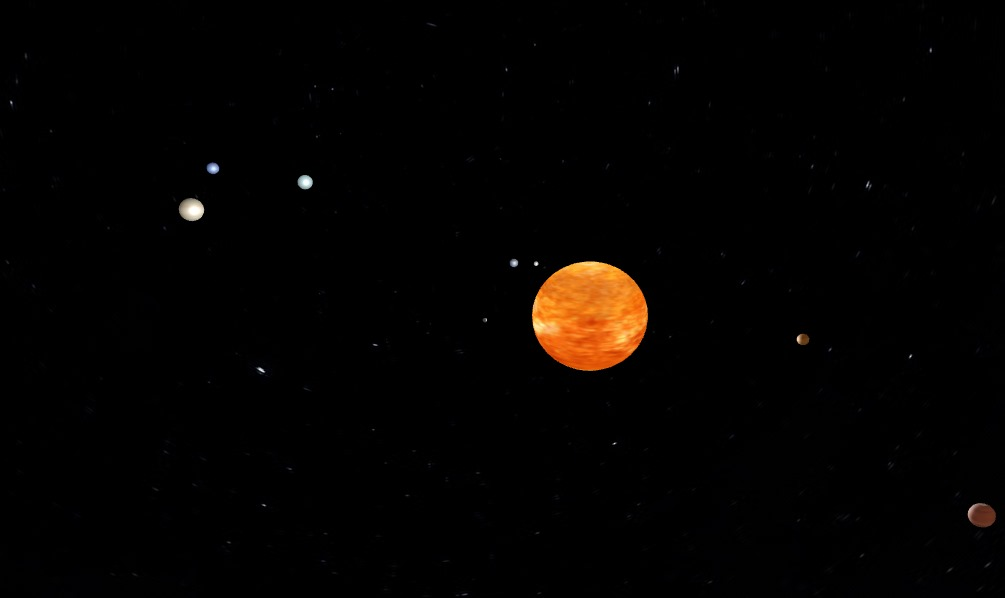
\includegraphics[width=300pt]{Sistema solar.jpg}
\caption{Sistema solar renderizado}
\end{figure}

\newpage

\subsection{Visualização de planetas e as suas sombras e os seus satelites em orbita}

\begin{figure}[!htb]
\centering
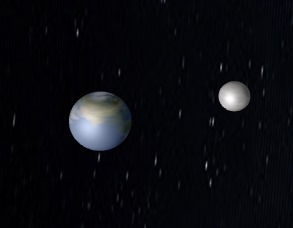
\includegraphics[width=300pt]{Terra.jpg}
\caption{Terra e a lua}
\end{figure}

\begin{figure}[!htb]
\centering
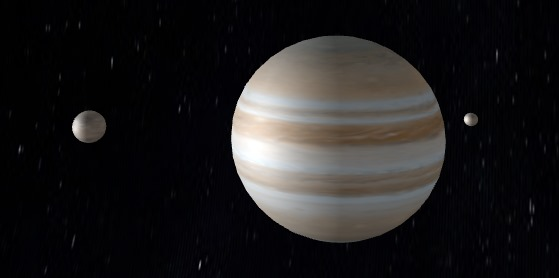
\includegraphics[width=300pt]{Saturno.jpg}
\caption{Saturno e os seus satelites}
\end{figure}

\newpage

\subsection{Visualização do ponto de reflexão dependendo de onde está posicionada a câmara.}


\begin{figure}[!htb]
\centering
\begin{minipage}{0.45\textwidth}
  \centering
  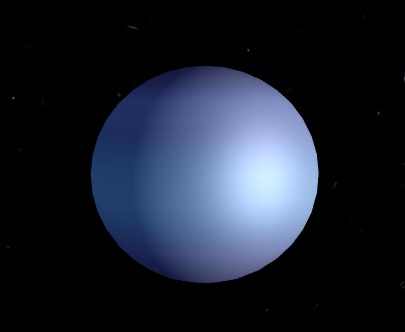
\includegraphics[width=1.2\linewidth]{luz1.jpg}
  \caption{Neptuno visto de lado}
\end{minipage}
\hfill
\begin{minipage}{0.45\textwidth}
  \centering
  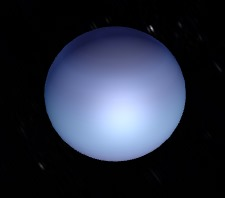
\includegraphics[width=1.115\linewidth]{luz2.jpg}
  \caption{Neptuno visto de frente}
\end{minipage}
\end{figure}


\newpage

\include{capitulo-5}

 \chapter{Trabalhos Futuros}
\label{chap:conclusao}
Num trabalho futuro, podemos considerar a implementação de elementos adicionais para enriquecer a experiência visual. Entre as possíveis adições, destacam-se a inclusão de menus iterativos, implementação da capacidade de desenhar as linhas das órbitas dos planetas, a representação detalhada do anel de Saturno, a reprodução visual da cintura de asteroides e a incorporação de controladores que permitam ajustar a velocidade das órbitas dos corpos celestes.

\section{Menus Iterativos}
A introdução de menus iterativos pode proporcionar uma interação mais dinâmica com o sistema solar simulado. Esses menus podem conter opções para explorar informações detalhadas sobre cada corpo celeste, como características físicas, dados históricos e curiosidades astronômicas.

\section{Linha das orbitras}

Integrar a representação visual das órbitas dos planetas acrescentaria um elemento gráfico essencial à simulação. Essas linhas podem ser desenhadas de forma elegante, destacando as trajetórias elípticas que os planetas percorrem em torno do Sol. A inclusão dessa característica não apenas aprimoraria a precisão da simulação, mas também ofereceria uma perspectiva mais intuitiva sobre os padrões de movimento orbital.

\newpage

\section{Anel de Saturno}
A adição do anel de Saturno ofereceria uma representação mais fiel e completa desse planeta fascinante. A modelagem precisa do anel, juntamente com a capacidade de ajustar a visibilidade e orientação do anel, seria uma contribuição valiosa para a simulação.

\section{Cintura de Asteroides}
A inclusão visual da cintura de asteroides entre as órbitas de Marte e Júpiter proporcionaria um elemento adicional de realismo à representação do sistema solar. Pode-se explorar opções para destacar asteroides significativos ou apresentar informações sobre composição e características individuais.

\section{Controladores de Velocidade}
A implementação de controladores interativos permitiria aos usuários ajustar a velocidade das órbitas dos planetas, proporcionando uma visão mais dinâmica do movimento celestial. Isso poderia ser realizado através de barras deslizantes ou caixas de diálogo que permitiriam a personalização da velocidade de rotação de cada corpo celeste.
Essas adições não apenas enriqueceriam a simulação, mas também proporcionariam uma experiência educativa mais envolvente, permitindo aos utulizadores explorar e compreender melhor os elementos do sistema solar de uma maneira interativa e informativa.

\chapter{Considerações Finais}

Ao chegarmos à conclusão do desenvolvimento deste projeto, experimentamos uma sensação de parcial satisfação, motivada pela conquista de praticamente todos os objetivos inicialmente propostos. Este percurso culminou em uma simulação cativante e realista do nosso sistema solar, proporcionando-nos uma visão envolvente dos movimentos celestiais que regem os corpos que compõem nosso sistema planetário.

Ao refletirmos sobre o tempo dedicado a esse empreendimento, ganhamos uma profunda apreciação pela importância intrínseca da Computação Gráfica (CG). A habilidade de visualizar e representar graficamente fenômenos astronômicos complexos ampliou consideravelmente nossa compreensão sobre o funcionamento interno do sistema solar. A complexidade dos cálculos orbitais, a aplicação de texturas realistas e a incorporação de elementos interativos, como menus e controladores, destacam-se como áreas nas quais a Computação Gráfica desempenha um papel crucial.

\clearpage{\thispagestyle{empty}\cleardoublepage}

\backmatter
\newpage



%\appendix
\bibliography{bibl}
\bibliographystyle{unsrt}
\nocite{UBI}
\nocite{ERD}

\end{document}
